
%(BEGIN_QUESTION)
% Copyright 2008, Tony R. Kuphaldt, released under the Creative Commons Attribution License (v 1.0)
% This means you may do almost anything with this work of mine, so long as you give me proper credit

A computer spreadsheet program may be used as a simulator for a PID controller.  By entering sets of values for Process Variable (PV), Setpoint (SP), Gain (K\_P), Integral time constant (tau\_I), Derivative time constant (tau\_D), and Bias (B), we may program a spreadsheet to calculate the controller output values and even graph them.

Begin creating your own spreadsheet by following the format shown below:

$$\includegraphics[width=15.5cm]{i03632x01.eps}$$

Assume a controller implementing the following P+D equation (note that our spreadsheet will calculate discrete steps rather than continuous change, hence the $\Delta$ notation instead of the more customary $d$ notation, and the summation symbol $\Sigma$ instead of the integration symbol $\int$):

$$\hbox{Output} = K_p e + {1 \over \tau_i} \Sigma (e \> \Delta t) + \tau_d {\Delta e \over \Delta t} + b$$

Write equations for spreadsheet cells in columns {\tt D}, {\tt E}, {\tt F}, and {\tt G} so that the error term, derivative term ($\tau_d {\Delta e \over \Delta t}$), integral term (${1 \over \tau_i} \Sigma (e \> \Delta t)$), and total output values will be automatically calculated for any PV and SP values entered in columns {\tt B} and {\tt C}.  Assume {\it direct action} for the controller.

\begin{itemize}
\item{} Formula for cell {\tt D3}:
\vskip 10pt
\item{} Formula for cell {\tt E3}:
\vskip 10pt
\item{} Formula for cell {\tt F3}:
\vskip 10pt
\item{} Formula for cell {\tt G3}:
\end{itemize}

Note: your first formula begins on row 3 rather than row 2 because you need to compare two points in time (e.g. row 3 versus row 2) in order to calculate rates of change and accumulated error-time products.  Simply enter zero (0) for the derivative term value in cell {\tt E2} as well as for the integral term value in cell {\tt F2}.

\underbar{file i03632}
%(END_QUESTION)





%(BEGIN_ANSWER)

\noindent
{\bf Partial answer:}

\begin{itemize}
\item{} Formula for cell {\tt D3}: = {\tt B3 $-$ C3}
\vskip 10pt
\item{} Formula for cell {\tt E3}: = {\tt \$I\$3 * (D3 $-$ D2) / (A3 $-$ A2)}
\vskip 10pt
\item{} Formula for cell {\tt F3}: = {\tt (D3 * (A3 $-$ A2) / \$I\$2) + F2}
\end{itemize}

%(END_ANSWER)





%(BEGIN_NOTES)

\begin{itemize}
\item{} Formula for cell {\tt D3}: = {\tt B3 $-$ C3}
\vskip 10pt
\item{} Formula for cell {\tt E3}: = {\tt \$I\$3 * (D3 $-$ D2) / (A3 $-$ A2)}
\vskip 10pt
\item{} Formula for cell {\tt F3}: = {\tt (D3 * (A3 $-$ A2) / \$I\$2) + F2}
\vskip 10pt
\item{} Formula for cell {\tt G3}: = {\tt (\$I\$1 * D3) + E3 + F3 + \$I\$4}
\end{itemize}

The dollar-sign symbols ({\tt \$}) are common Excel formatting for absolute cell coordinates.  This is important when cell formulae are copied and duplicated on other columns and/or other rows.  If absolute coordinates are not given for the gain and bias values, the copied formulae on rows 3 and up will be incorrectly referenced.


%INDEX% Control, proportional + integral + derivative: graphing controller response
%INDEX% Computer spreadsheet exercise: proportional+integral+derivative controller response

%(END_NOTES)


